\chapter{The Internet}

% \section*{Overview}
The Internet is a global network of interconnected computer networks that use standardized communication protocols. This unit covers core concepts about how the Internet works and its impact on society.


\section*{Learning Objectives}

\subsection*{The Internet (4.1)}
\begin{itemize}[label=--]
    \item \textbf{CSN-1.A}: Explain how devices communicate in a network. % CSN-1.A
    \item \textbf{CSN-1.B}: Understand the structure and functionality of the Internet. % CSN-1.B
    \item \textbf{CSN-1.C}: Explain data transmission via packets. % CSN-1.C
    \item \textbf{CSN-1.D}: Differentiate between the Internet and the World Wide Web. % CSN-1.D
\end{itemize}

\subsection*{Fault Tolerance (4.2)}
\begin{itemize}[label=--]
    \item \textbf{CSN-1.E}: Understand and describe fault tolerance in networks. % CSN-1.E
\end{itemize}

\subsection*{Digital Divide (5.2)}
\begin{itemize}[label=--]
    \item \textbf{IOC-1.C}: Describe issues that contribute to the digital divide. % IOC-1.C
\end{itemize}

\section*{Essential Knowledge}

\subsection*{The Internet (4.1)}

\begin{itemize}
    \item \textbf{Computing Devices and Networks}
        \begin{itemize}
            \item \textbf{Computing Device}: Physical tools (e.g., computers, routers) capable of running programs. % CSN-1.A.1
            \item \textbf{Computing System}: A collaborative group of devices and programs with a common purpose. % CSN-1.A.2
            \item \textbf{Computer Network}: Interconnected devices that can send and receive data, like the Internet. % CSN-1.A.3
            \item \textbf{Network Path}: Route taken by data between two devices in a network, involving a series of directly connected devices. % CSN-1.A.5
            \item \textbf{Routing}: The process of selecting a path for data in a network from sender to receiver. % CSN-1.A.6
            \item \textbf{Bandwidth}: The maximum data volume that can be sent over a network in a given time, usually measured in bits per second. % CSN-1.A.7, CSN-1.A.8
        \end{itemize}

    \item \textbf{Internet Structure and Protocols}
        \begin{itemize}
            \item \textbf{Internet}: A global network of interconnected networks that communicate using standardized, open protocols. % CSN-1.B.1
            \item \textbf{Protocol}: Agreed-upon rules that dictate how data is transmitted; open protocols allow for easy connectivity and interoperability of devices. % CSN-1.B.3
            \item \textbf{Dynamic Routing}: Internet paths are flexible and often change based on network conditions. % CSN-1.B.5
            \item \textbf{Scalability}: The Internet’s design allows it to grow and adapt to meet increasing demand. % CSN-1.B.6
        \end{itemize}

    \item \textbf{Data Transmission Through Packets}
        \begin{itemize}
            \item \textbf{Data Stream}: Continuous flow of data transmitted as a series of packets. % CSN-1.C.1
            \item \textbf{Packet}: A small unit of data that includes payload (data) and metadata (information for routing and reassembly). % CSN-1.C.2
            \item \textbf{Packet Protocols}: Common protocols include IP, TCP, and UDP, which manage data routing and delivery. % CSN-1.C.4
        \end{itemize}

    \item \textbf{Internet vs. World Wide Web}
        \begin{itemize}
            \item \textbf{World Wide Web (WWW)}: A system of interconnected pages and files accessible via the Internet. % CSN-1.D.1
            \item \textbf{HTTP Protocol}: The protocol that enables communication on the Web. % CSN-1.D.2
            \item \textbf{Relationship}: The Web relies on the Internet to operate but is a separate service layer. % CSN-1.D.3
        \end{itemize}
\end{itemize}

\subsection*{Fault Tolerance (4.2)}

\begin{itemize}
    \item \textbf{Fault Tolerance}: The Internet is designed to withstand failures, maintaining functionality when parts of the network fail. % CSN-1.E.1
    \item \textbf{Redundancy}: Extra components, like alternate paths, ensure data can reroute around issues, enhancing reliability. % CSN-1.E.2, CSN-1.E.3
    \item \textbf{Resilience}: Redundancy enables fault tolerance, allowing the network to continue operating despite failures. % CSN-1.E.5, CSN-1.E.6
\end{itemize}


\begin{figure}[h!]
    \centering
    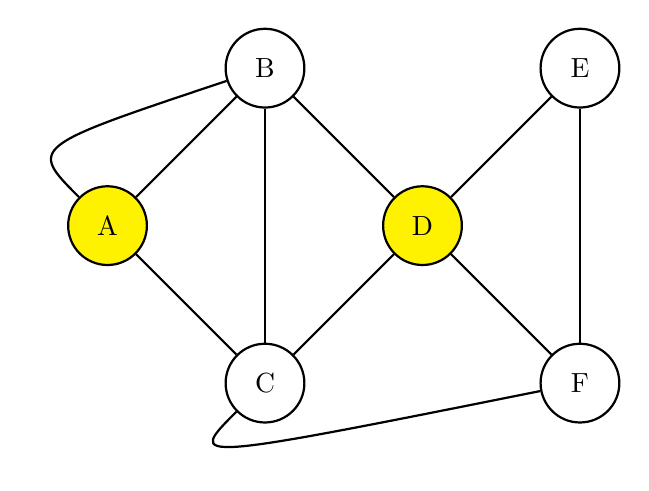
\begin{tikzpicture}[every node/.style={circle, draw, minimum size=1cm, inner sep=0pt}, 
                        thick]
        % Define nodes with highlighted A and D
        \node[fill=yellow] (A) at (0,0) {A};
        \node (B) at (2,2) {B};
        \node (C) at (2,-2) {C};
        \node[fill=yellow] (D) at (4,0) {D};
        \node (E) at (6,2) {E};
        \node (F) at (6,-2) {F};
        
        % Define undirected connections
        \draw (A) -- (B);
        \draw (A) -- (C);
        \draw (B) -- (C);
        \draw (B) -- (D);
        \draw (C) -- (D);
        \draw (D) -- (E);
        \draw (D) -- (F);
        \draw (E) -- (F);
        
        % Additional paths for redundancy
        \draw (A) .. controls (-1, 1) .. (B);
        \draw (C) .. controls (1, -3) .. (F);
        
    \end{tikzpicture}
    \captionsetup{list=no}
    \caption{
        This network diagram demonstrates key concepts in network design:\protect\\
        • Path: A route data can take from one node to another. Here, multiple paths connect nodes \textbf{A} and \textbf{D}.\protect\\
        • Redundancy: Multiple paths between nodes (like from \textbf{A} to \textbf{D} via \textbf{B} or \textbf{C}) provide backup routes.\protect\\
        • Fault Tolerance: If one path breaks, the network still works because of backup paths.\protect\\
        Nodes \textbf{A} and \textbf{D} are highlighted to show an example of endpoint devices in a network path.
    }
\end{figure}


% \section{Internet Architecture}
% \begin{itemize}
%     \item \textbf{Devices}: Computers, routers, switches, and servers
%     \item \textbf{Packets}: Small units of data that travel across networks
%     \item \textbf{Bandwidth}: Maximum data transfer rate of a network
% \end{itemize}

% \begin{figure}[h]
%     \centering
%     \begin{tikzpicture}[
%         box/.style={
%             draw,
%             rectangle,
%             minimum width=8cm,
%             minimum height=1.5cm,
%             text width=7.5cm,
%             align=center,
%             fill=gray!10
%         }
%     ]
%         % Layer boxes
%         \node[box] (app) at (0,6) {Application Layer\\(HTTP, DNS, FTP)};
%         \node[box] (transport) at (0,4) {Transport Layer\\(TCP, UDP)};
%         \node[box] (internet) at (0,2) {Internet Layer\\(IP)};
%         \node[box] (link) at (0,0) {Link Layer\\(Ethernet, WiFi)};
        
%         % Arrows between layers
%         \draw[->,thick] (app.south) -- (transport.north);
%         \draw[->,thick] (transport.south) -- (internet.north);
%         \draw[->,thick] (internet.south) -- (link.north);
        
%         % Add labels on the right
%         \node[align=left] at (5,6) {Web browsing,\\email, file transfer};
%         \node[align=left] at (5,4) {End-to-end\\communication};
%         \node[align=left] at (5,2) {Addressing and\\routing};
%         \node[align=left] at (5,0) {Physical\\transmission};
        
%     \end{tikzpicture}
%     \caption{The four layers of the Internet protocol suite}
%     \label{fig:network-layers}
% \end{figure}

% \section{Protocols}
% \begin{itemize}
%     \item \textbf{TCP/IP}: Core protocols for reliable data transmission
%     \item \textbf{HTTP/HTTPS}: Web communication protocols
%     \item \textbf{DNS}: Domain Name System for converting URLs to IP addresses
% \end{itemize}

% \section{Addressing and Routing}
% \begin{itemize}
%     \item \textbf{IP Addresses}: Unique identifiers for devices (IPv4, IPv6)
%     \item \textbf{Routing}: How data finds its path across networks
%     \item \textbf{Domain Names}: Human-readable web addresses
% \end{itemize}

% \section{Cybersecurity}
% \begin{itemize}
%     \item \textbf{Common Threats}:
%         \begin{itemize}
%             \item Phishing: Deceptive attempts to steal user data
%             \item DDoS: Distributed Denial of Service attacks
%             \item Malware: Malicious software types
%         \end{itemize}
%     \item \textbf{Protection Methods}:
%         \begin{itemize}
%             \item Encryption: Securing data transmission
%             \item Authentication: Verifying user identity
%             \item Updates: Maintaining system security
%         \end{itemize}
% \end{itemize}

\subsection*{Digital Divide (5.2)}

\begin{itemize}
    \item Refers to differing access to computing devices and the Internet based on socioeconomic, geographic, or demographic characteristics % IOC-1.C.2
    \item Access varies between countries and demographic groups % IOC-1.C.1
    \item Affects both groups and individuals % IOC-1.C.3
    \item Raises issues of equity, access, and influence globally and locally % IOC-1.C.4
    \item Influenced by actions of individuals, organizations, and governments % IOC-1.C.5
\end{itemize}

\subsection*{Other Topics on Code.org}
\begin{itemize}
    \item \textbf{Net Neutrality}: Principle that Internet Service Providers should treat all Internet traffic equally, without discriminating based on content or source
    \item \textbf{Internet Censorship}: Government or organizational control over Internet access and content, which can limit free speech and information flow
\end{itemize}